\chapter{Forundersøgelse}\label{ch:forundersoegelse}
Nu hvor virksomheden er blevet undersøgt og hovedproblemerne er opsat, kan der nu laves en undersøgelse af, hvilke use cases der skal integreres i systemet. De opgaver, som er stillet op fra konklusionen på business analysen, er automatisk lagerstyring, integration af ordre i systemet og automatisk bogføring. Af de tre opgaver her fravælges integration af ordre, da der også skulle integreres et ruteplanlægningssystem, hvilket er dømt til at være for stor en opgave. Første prioritet er i stedet automatisk lagerstyring, og anden prioritet er automatisk bogføring.

\section{Workflow Diagrammer}

Der er lavet Workflow diagrammer \cite{Workflow} for de opgaver der bliver udført hos Hjem-IS Aalborg depotet nu. Disse diagrammer kan ses i Figur~\ref{fig:workflows}. Disse workflows beskriver i store træk, hvilke trin der er i opgaverne. Disse workflows vil også blive brugt til at finde ud af, hvilke af opgaverne der skal bruges og laves om, så det kan passe til et nyt system. Eftersom salg af is ude ved kunderne ikke er en Use Case på selve depotet, tages den ikke med her.

\begin{figure}[p]
    \centering
    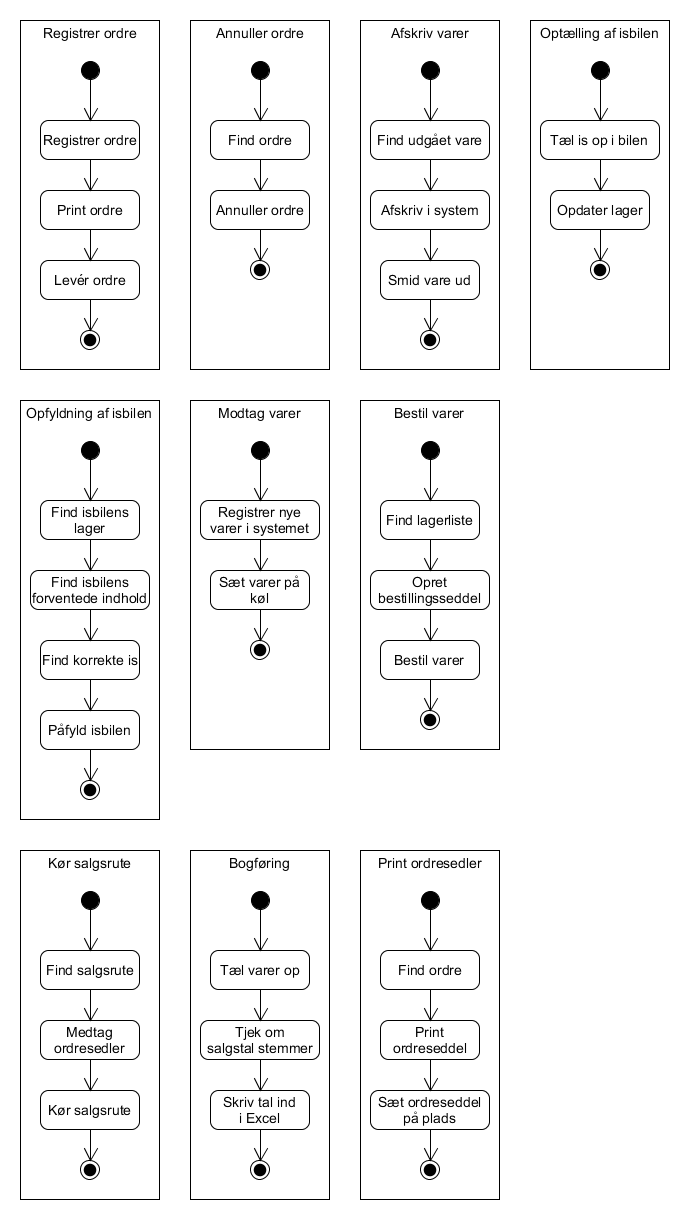
\includegraphics[width=0.9\textwidth]{figures/Forundersøgelse/workflows.png}
    \caption{Workflow diagram}
    \label{fig:workflows}
\end{figure}

De workflows der skal bruges til at kunne lave automatisk lagerstyring er Bestil Vare, Modtag Vare, Optælling af isbilen og Afskriv vare. Alle disse trin er nødvendige for at der kan laves en forudsigelse af, hvor mange varer der skal bestilles hjem. For at det kan lade sig gøre at lave et estimat for hvor mange af hvert produkt, der skal bestilles hjem, kræves det at der i forvejen er et lager med varer, og mindst én dags salgsstatistik tilgængelig. Det er vigtigt at lave optælling af isbilen for at dobbelttjekke at lageret passer - det er trods alt den data der bruges, til at bedømme hvor meget der skal bestilles hjem. Såfremt en vare skal afskrives, så skal lageret også opdateres så det stemmer. Til sidst skal der selvfølgelig bestilles varer, som så skal modtages og registreres som værende på lager. For at udpensle trinene i opgaverne laves der en medarbejder-mål-tabel over de workflows, der er opstillet i figur \ref{fig:workflows}.

\section{Medarbejder-mål Tabel}
Ud fra Workflowet er der opstillet en medarbejder-mål tabel \cite{Larman2004}. Dens formål er at belyse de arbejdsopgaver, der er hos Hjem-IS, samt give et indblik i, hvilke behov der skal opfyldes for, at finde krav til et automatisk lagerstyringssystem.
Nedenfor er der udarbejdet medarbejder-mål tabellen. Den er opdelt i fire rækker som består af; "Medarbejder", "Opgave", "Mål", og "Trin".
"Medarbejder" er rækken hvor man beskriver, hvilken aktør, der skal udføre en eller flere handlinger (f.eks. Ismand). Der er ikke kun én rolle hos Hjem-IS, så det er vigtigt at få udpeget hvem, der udfører hvad.
"Opgave" rækken viser de opgaver, som skal udføres af aktøren på samme linje. Det er som regel meget vigtige opgaver, som er relevante for Hjem-IS' drift.
"Mål" er det endelige resultat af aktørens handlinger i opgaven.
"Trin" viser en oversigt over hver handling, som aktøren skal udføre for at komme fra den udvalgte opgave, til det endelige mål. Trinene er med til at vægte hvor kompleks opgaven er, som der så kan tages med til overvejelse, når der skal laves Use Cases.

\begin{center}
\begin{longtable}{ |p{90pt}|p{90pt}|p{90pt}|p{90pt}| }
    \hline
    Medarbejder & Opgave & Mål & Trin \\
    \hline\hline
    Ismand
    & Modtager ny ordre & Ordren er registreret som værende solgt. &
    - Modtag ordre fra kunde \\
    &&&
    - Ordren med tilhørende adresse registreres \\
    &&&
    - Ordren med adressen printes ud og lægges i den rigtige kasse til næste dag \\
    &&&
    - Den udprintede ordre tages med i bilen \\
    &&&
    - Ordren leveres til kunden på turen \\
    &&&
    - Kunden underskriver ordren \\
    &&&
    - Den underskrevne ordre afleveres til chefen efter turen er færdig \\
    \hline
    Ismand & Annuller ordre & Ordren er annulleret &
    - Modtag ordre fra kunde \\
    &&&
    - Under “registrer ordre”, før samtlige trin er gennemført, kontakter kunden depotet og vil have en ordre annulleret \\
    &&&
    - Ordren annulleres. \\
    \hline
    Lagermedarbejder
    & Isbilen skal ryddes op & Isbilens bokse er ryttet op så der er plads til nye varer &
    - Ismanden åbner en boks med is \\
    &&&
    - Ismanden omrokerer pakkerne således at der er bedre plads til nye pakker næste dag \\
    &&&
    - Ismanden lukker boksen \\
    &&&
    - Gentages indtil alle bokse er ryddet op. \\
    \hline
    Lagermedarbejder
    & Modtager nye varer & Varerne er registreret og lagt i fryseren &
    - Nye varer ankommer til depotet \\
    &&&
    - Varerne læsses af på paller \\
    &&&
    - Varerne registreres og godkendes så mængden stemmer \\
    &&&
    - Varerne lægges ind i fryseren \\
    \hline
    Lagermedarbejder & Varer skal afskrives & Varer er afskrevet &
    - Lageret er blevet talt op \\
    &&&
    - Under optælling er der fundet varer, som er udløbet \\
    &&&
    - Varerne tilsidesættes \\
    &&&
    - Varerne registreres som udløbet i systemet \\
    &&&
    - Varerne er afskrevet og kan ikke sælges \\
    \hline
    Ismand & Isbilen skal ryddes op & Isbilens bokse er ryttet op så der er plads til nye varer & 
    - Ismanden åbner en boks med is \\
    &&&
    - Ismanden omrokerer pakkerne således at der er bedre plads til nye pakker næste dag \\
    &&&
    - Ismanden lukker boksen \\
    &&&
    - Gentages indtil alle bokse er ryddet op. \\
    \hline
    Lagermedarbejder & Isbilen skal påfyldes med is & Isbilen er påfyldt & 
    - Lagermedarbejder modtager bestillingsseddel, hvorpå der står hvor meget der skal fyldes på de forskellige biler. \\
    &&&
    - Lagermedarbejder fylder isene på en vogn inde i fryseren og kører herefter vognen ud til isbilen og fylder på. \\
    \hline
    Bogfører (chef) & Mindstemængderne af isene skal opdateres & Mindstemængderne af isene er opdateret &
    - Først undersøges hvilke is der har solgt godt og mindre godt \\
    &&&
    - Der laves en evaluering ud fra antallet solgt og nuværende mindstemængde på hver is \\
    &&&
    - Efter en manuel vurdering opdateres mindstemængderne så det passer til efterspørgslen. \\
    \hline
    Bogfører (chef) & Is skal bestilles hjem ud fra hvor mange is der mindst skal være på lager, og hvor mange is der skal være i hver bil & Is er bestilt hjem, i henhold til den manuelle vurdering af hvor mange der skal være. &
    - Undersøg hvor mange af hver is der blev solgt dagen før \\
    &&&
    - Lav en manuel vurdering af om mindstemængderne er i orden \\
    &&&
    - Lav en manuel vurdering af om nuværende antal på lageret er i orden \\
    &&&
    - Foretag ændringer af mindstemængder \\
    &&&
    - Bestil nye is hjem ud fra vurderingen så der er nok til næste gang \\
    \hline
    Ismand & Modtag nyt salg på ruten & Salget er registreret & 
    - På ruten kommer en kunde forbi bilen og vil købe is \\
    &&&
    - Ismanden finder de ønskede varer \\
    &&&
    - Varerne tilføjes til salget \\
    &&&
    - Kundeoplysninger tilføjes til salget \\
    &&&
    - Salget afsluttes \\
    &&&
    - Ordrebekræftelse til kunde, lager og regnskab \\
    \hline
    Chef & Medarbejderen skal evalueres hver måned & Medarbejderen er evalueret &
    - Medarbejderens præstationer ud fra målene læses \\
    &&&
    - Der laves en vurdering af hvilke områder medarbejderen skal fokusere på at gøre bedre \\
    &&&
    - Medarbejderen indkaldes til en samtale \\
    &&&
    - Medarbejderen for at vide hvilke områder der skal forbedres \\
    \hline
    Bogfører (chef) & Alle salg for dagen er afsluttet & Alle salgstal er bogført & 
    - Find all tallene for dagen \\
    &&&
    - Åben et Excel dokument til bogføring \\
    &&&
    - Manuelt skriv af til excel dokumentet \\
    &&&
    - Gem dokumentet. \\
    \hline
\end{longtable}
\end{center}

\section{Use Case Diagram}\label{usecase}
I Figure~\ref{fig:usecasediagram} ses der et use case diagram lavet ud fra medarbejder-mål tabellen. Use case diagrammet giver et godt overblik over, hvilke opgaver de forskellige aktører udfører mellem aktør og system \cite{visual-paradigm.com}. 

\begin{figure}[p]
    \centering
    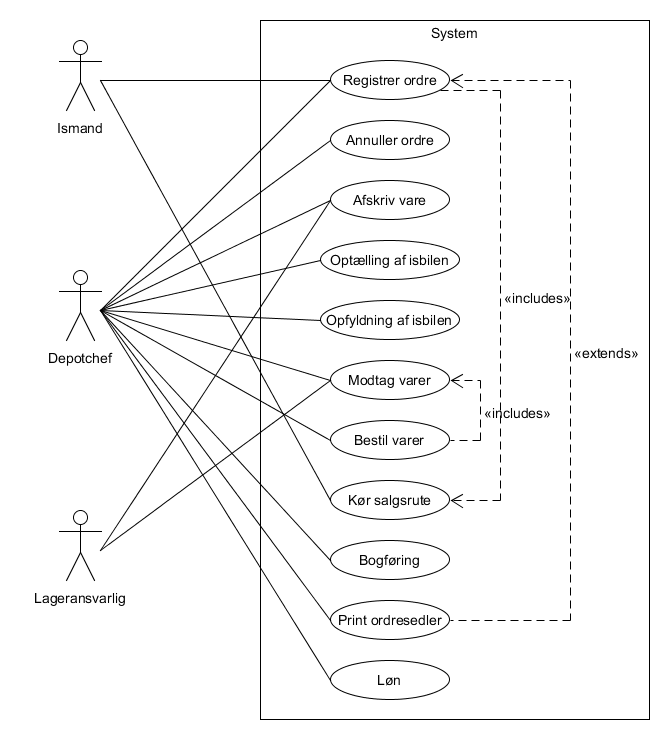
\includegraphics[width=0.9\textwidth]{figures/Forundersøgelse/use_case_diagram.png}
    \caption{Use Case diagram}
    \label{fig:usecasediagram}
\end{figure}

Use Case diagrammet viser at depotchefen står for næsten alle opgaver i virksomheden. Depotchefen udtrykte en interesse for at kunne bruge mindre tid på de mange opgaver, han har i løbet af dagen, for så at kunne bruge tid på at køre salgsruter. Eftersom det også primært er depotchefen, der står for de opgaver, som udføres i systemet, er det de Use Cases der vil blive fokuseret på.

\section{Brief Use Cases}\label{brief}
\textbf{Register ordre:}\label{briefreg} \\
En ordre modtages, på hjemmesiden. Alt afhængig af hvor ordren registreres, vil den blive sendt ud til det nærmeste depot. F.eks hvis ordren er fra Nordjylland, er det depotet i Aalborg, som har ansvaret for at ordren skal leveres. Herfra modtager chefen ordren og registerer den, efterfuldt af dette, vil en printet seddel gives til en sælger, som registere ordren, når den bliver afleveret til kunden. 

\textbf{Annuller ordre:}\label{briefcancel} \\
En kunde fortryder sin ordre, herfra kan kunden annullere orderen

\textbf{Afskriv vare:}\label{briefremove} \\
En lagermedarbejder finder en udgået vare og belyser depotchefen, som afskriver det i systemet. Herfra kan lagermedarbejderen smide varen ud. 

\textbf{Optælling af isbilen:}\label{briefcount} \\
Depot chefen tæller isbilen op, noterer det ned og opdaterer lageret. 

\textbf{Modtag varer:}\label{briefreceive} \\
En lagermedarbejder modtager varerne, når lastbilerne fylder fryseren ud. Herfra registeres de modtagede varer. 

\textbf{Bestil varer:}\label{brieforder} \\
Depotchefen holder øje med depotets fryser og fylder ud, når der er mangel på bestemt varer. Udover dette bestiller depotchefen flere af en bestemt vare hjem, når der er tilbud på en bestemt vare. 

\textbf{Kør salgsrute:}\label{briefdrive} \\
En sælger modtager den bestemte rute, som sælgeren skal køre. Herfra indtaster sælgeren ruten ind i rutesystemet. Systemet finder ruten og nu er sælgeren klar til at køre ud med is. 

\textbf{Bogføring:}\label{briefbook} \\
Depotchefen tæller varene op, optæller om salgstallet stemmer overens. Herfra tastes tallene ind i excel. 

\textbf{Print ordrersedler:}\label{briefprint} \\
Depotchefen finder ordren og printer den ud. Herfra lægges den udprintede ordre på en hylde, som passer bedst med en af de kommende ruter.

\section{Mock ups og designprincipper}\label{sec:mockup}
Når det kommer til at designe en brugergrænseflade til sit system, er der optil flere overvejelser man skal igennem. Målet er at gøre brugergrænsefladen brugervenlig, hurtig og intuitiv. Dette afsnit vil derfor gennemgå hvilke overvejelser, der er indgået i beslutningen for designet af de anvendte mock ups, som kan ses på bilag \ref{app:mockups}.

\subsection{User Groups og Personas}
Som det første kan det hurtig etableres, at brugeren af systemet primært bliver depotchef Niels Thomas, da opgaverne der skal laves med brug af systemet primært er hans. Brugergruppen det vedrører, er derfor en gruppe fra fyrre og op efter, som ikke meget interneterfaring har, og hvis mulighed for at lære nye ting også er begrænset. Brugergruppen kan dog finde ud af at bruge de forskellige internetsider og systemer, der bruges til dagligt på arbejdspladsen, og han er derfor allerede bekendt med opgaverne samt hvordan de skal udføres. 

Knapperne og teksten skal være designet til at være store letlæselige bogstaver, høj kontrast mellem baggrunden og knapperne. Trinene og knap-placeringerne er intuitive, så det ikke er svært at lære.
Det forventes at farvepaletten og skrifttypen stemmer overens med Hjem-IS' hjemmeside \cite{hjemis}. Eftersom Niels Thomas under interviewet har udtrykt et ønske om at kunne spare tid på sine opgaver, er det vigtigt at forståelse for systemet er en kort process. Derfor vil Niels Thomas også have en forventning til, at det nye system skal kunne være nemt at bruge, så det lykkedes at opfylde ønsket.

\subsection{Skrifttype}\label{skrifttype}
Skrifttypen Segoe UI Black er valgt fordi den minder meget om skrifttypen anvendt på Hjem-IS' hjemmeside \cite{hjemis}. Skrifttypen er tyk, rund og ikke så skarp, hvilket gør den nem og behagelig at læse. Skrifttypen reflekterer også den afslappede og uformelle kultur Hjem-IS har.

